\documentclass[]{article}
\usepackage{lmodern}
\usepackage{amssymb,amsmath}
\usepackage{ifxetex,ifluatex}
\usepackage{fixltx2e} % provides \textsubscript
\ifnum 0\ifxetex 1\fi\ifluatex 1\fi=0 % if pdftex
  \usepackage[T1]{fontenc}
  \usepackage[utf8]{inputenc}
\else % if luatex or xelatex
  \ifxetex
    \usepackage{mathspec}
  \else
    \usepackage{fontspec}
  \fi
  \defaultfontfeatures{Ligatures=TeX,Scale=MatchLowercase}
\fi
% use upquote if available, for straight quotes in verbatim environments
\IfFileExists{upquote.sty}{\usepackage{upquote}}{}
% use microtype if available
\IfFileExists{microtype.sty}{%
\usepackage{microtype}
\UseMicrotypeSet[protrusion]{basicmath} % disable protrusion for tt fonts
}{}
\usepackage[margin=1in]{geometry}
\usepackage{hyperref}
\hypersetup{unicode=true,
            pdftitle={Motor Trend - MPG Comparison},
            pdfborder={0 0 0},
            breaklinks=true}
\urlstyle{same}  % don't use monospace font for urls
\usepackage{longtable,booktabs}
\usepackage{graphicx,grffile}
\makeatletter
\def\maxwidth{\ifdim\Gin@nat@width>\linewidth\linewidth\else\Gin@nat@width\fi}
\def\maxheight{\ifdim\Gin@nat@height>\textheight\textheight\else\Gin@nat@height\fi}
\makeatother
% Scale images if necessary, so that they will not overflow the page
% margins by default, and it is still possible to overwrite the defaults
% using explicit options in \includegraphics[width, height, ...]{}
\setkeys{Gin}{width=\maxwidth,height=\maxheight,keepaspectratio}
\IfFileExists{parskip.sty}{%
\usepackage{parskip}
}{% else
\setlength{\parindent}{0pt}
\setlength{\parskip}{6pt plus 2pt minus 1pt}
}
\setlength{\emergencystretch}{3em}  % prevent overfull lines
\providecommand{\tightlist}{%
  \setlength{\itemsep}{0pt}\setlength{\parskip}{0pt}}
\setcounter{secnumdepth}{0}
% Redefines (sub)paragraphs to behave more like sections
\ifx\paragraph\undefined\else
\let\oldparagraph\paragraph
\renewcommand{\paragraph}[1]{\oldparagraph{#1}\mbox{}}
\fi
\ifx\subparagraph\undefined\else
\let\oldsubparagraph\subparagraph
\renewcommand{\subparagraph}[1]{\oldsubparagraph{#1}\mbox{}}
\fi

%%% Use protect on footnotes to avoid problems with footnotes in titles
\let\rmarkdownfootnote\footnote%
\def\footnote{\protect\rmarkdownfootnote}

%%% Change title format to be more compact
\usepackage{titling}

% Create subtitle command for use in maketitle
\newcommand{\subtitle}[1]{
  \posttitle{
    \begin{center}\large#1\end{center}
    }
}

\setlength{\droptitle}{-2em}

  \title{Motor Trend - MPG Comparison}
    \pretitle{\vspace{\droptitle}\centering\huge}
  \posttitle{\par}
    \author{}
    \preauthor{}\postauthor{}
    \date{}
    \predate{}\postdate{}
  

\begin{document}
\maketitle

\hypertarget{executive-summary}{%
\subsubsection{Executive Summary}\label{executive-summary}}

Miles per gallon (MPG) is an important metric for any person considering
to buy a car. Motor trend magazine has collected data from a series of
cars to understand how different car attirbutes affect MPG.
Specifically, we are interestd in understanding:

\begin{enumerate}
\def\labelenumi{\arabic{enumi}.}
\tightlist
\item
  Is an automatic or manual transmission better for MPG?
\item
  How much difference is there between automatic and manual transmission
  for MPG consumption?
\end{enumerate}

The analysis concluded that: - automatic cars have a lower MPG. - but
this analysis is limited by confounding variables such as weight which
could influence the results.

\hypertarget{exploring-the-data}{%
\subsubsection{Exploring the data}\label{exploring-the-data}}

We collected 32 observations to inform our study:

\begin{longtable}[]{@{}lrr@{}}
\caption{Summary of observations}\tabularnewline
\toprule
transmission & Number of Observations & Mean MPG\tabularnewline
\midrule
\endfirsthead
\toprule
transmission & Number of Observations & Mean MPG\tabularnewline
\midrule
\endhead
automatic & 19 & 17.15\tabularnewline
manual & 13 & 24.39\tabularnewline
\bottomrule
\end{longtable}

To understand how transmission type effects MPG, we can compare the MPG
observation between the two transmission types. From an initial
comparison, it looks clear that automatic cars have a better (lower) MPG
result than manual transmission cars.

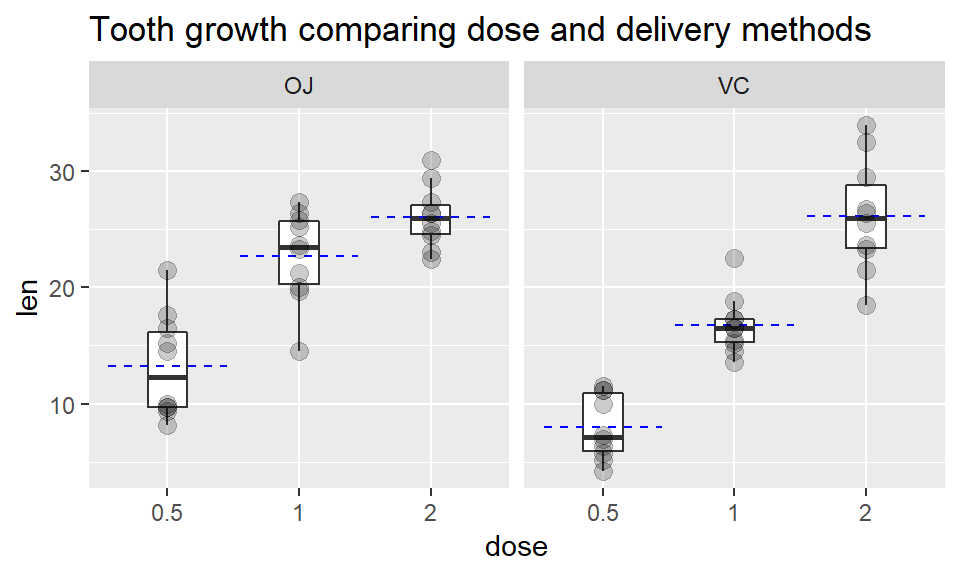
\includegraphics{Week_4_-_Project__Motor_Trend_Report__v1.1_files/figure-latex/unnamed-chunk-3-1.pdf}

We will now fit several models to understand if the difference is
statistically signifcant, and if the method of predicing MPG using
transmission type is useful.

\hypertarget{model-1}{%
\subsubsection{Model \#1}\label{model-1}}

Our first model will consider only MPG and transmission type. Using this
simple model, we predict that:

\begin{itemize}
\tightlist
\item
  if a car is automatic it will have a MPG of 17.1474
\item
  if a car is manual it will have a mean of 24.3923
\end{itemize}

The model also shows us that:

\begin{itemize}
\item
  a low p-value indicates that the the difference is statistically
  signifcant
\item
  r-squared of 0.3598 means that there is still a lot of variance not
  yet exlpained by the model

  \begin{longtable}[]{@{}lllrl@{}}
  \toprule
  & Estimate S & td. Error & t value P &
  r(\textgreater{}\textbar{}t\textbar{})\tabularnewline
  \midrule
  \endhead
  (Intercept) & 17.147368 & 1.124602 & 15.247492 &
  0.000000\tabularnewline
  transmissionmanual & 7.244939 & 1.764422 & 4.106127 &
  0.000285\tabularnewline
  \bottomrule
  \end{longtable}
\end{itemize}

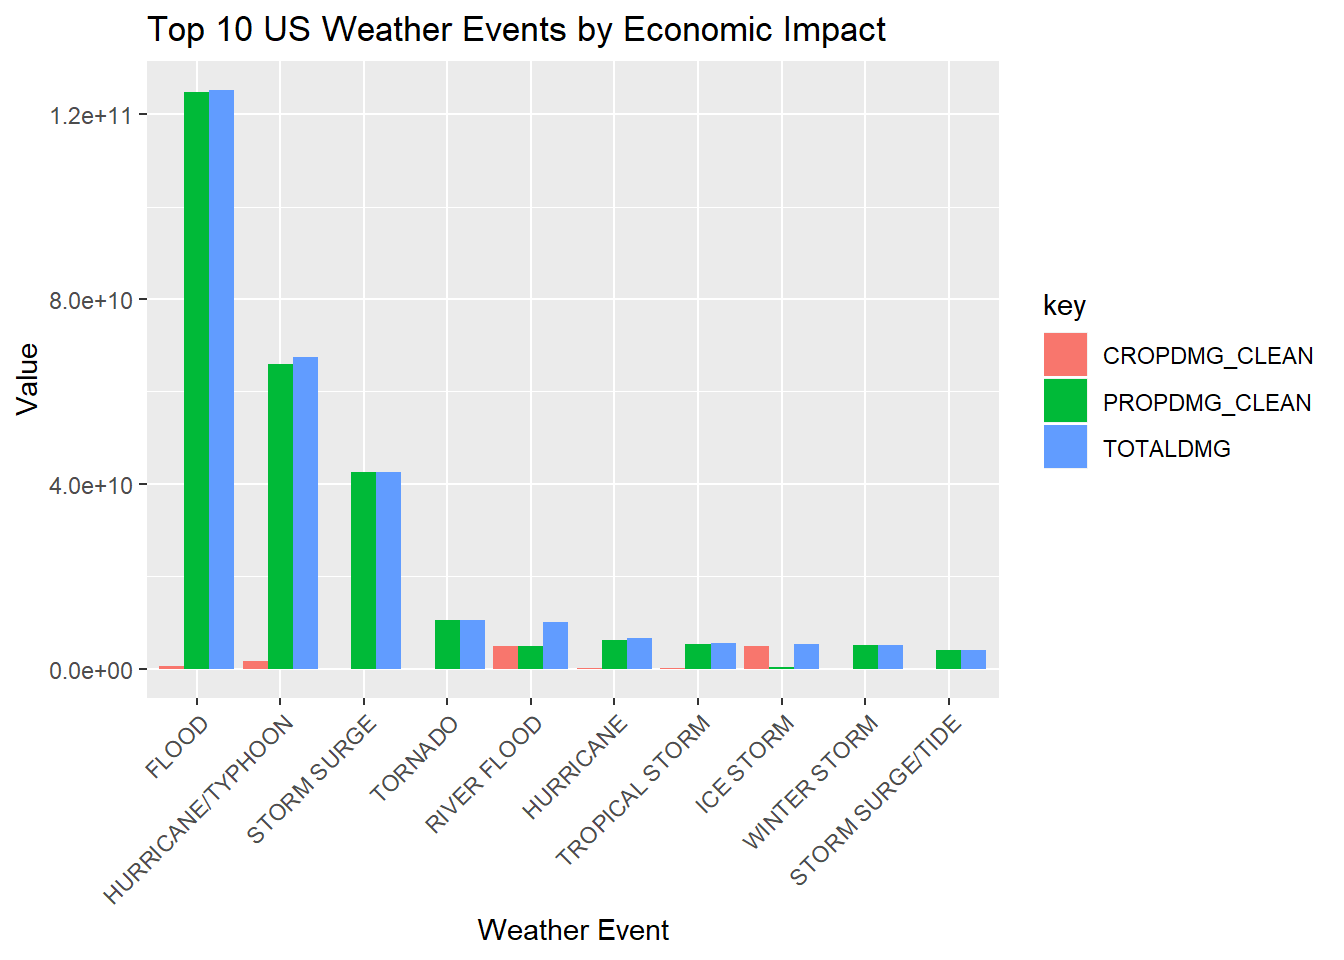
\includegraphics{Week_4_-_Project__Motor_Trend_Report__v1.1_files/figure-latex/unnamed-chunk-6-1.pdf}

\hypertarget{model-2}{%
\subsubsection{Model \#2}\label{model-2}}

With model \#2 we will seek to explain more of the variance by
introducing more variables into the model. With the introduction of
weight interacting on transmission, our model now tells us that:

\begin{itemize}
\tightlist
\item
  r-squared of 0.833 means that most of the variance is explained by the
  model
\item
  the residual plot shows no patterns in the data, supporting the model
  is appropriate
\item
  for automatic transmission cars:

  \begin{itemize}
  \tightlist
  \item
    the intercept of 31.4160554 is the MPG at the theoretical weight of
    0
  \item
    for each 1000lb increase in weight, MPG will change by -3.7859075
  \end{itemize}
\item
  for manual transmition cars:

  \begin{itemize}
  \tightlist
  \item
    the intercept of 46.2944779 is the MPG at the theoretical weight of
    0
  \item
    for each 1000lb increase in weight, MPG will change by -9.084268
  \end{itemize}
\end{itemize}

One limitation of this model is that there is not a lot of overlap in
weight between manual and automatic transmission cars. Generally, manual
cars tend to be heavier which also correlates a lower MPG. For example
at lighter weights manual cars have a lower MPG.

\begin{longtable}[]{@{}lrrrr@{}}
\toprule
& Estimate & Std. Error & t value &
Pr(\textgreater{}\textbar{}t\textbar{})\tabularnewline
\midrule
\endhead
(Intercept) & 31.416055 & 3.0201093 & 10.402291 &
0.0000000\tabularnewline
wt & -3.785907 & 0.7856478 & -4.818836 & 0.0000455\tabularnewline
transmissionmanual & 14.878422 & 4.2640422 & 3.489276 &
0.0016210\tabularnewline
wt:transmissionmanual & -5.298361 & 1.4446993 & -3.667449 &
0.0010171\tabularnewline
\bottomrule
\end{longtable}

\includegraphics{Week_4_-_Project__Motor_Trend_Report__v1.1_files/figure-latex/unnamed-chunk-9-1.pdf}

\includegraphics{Week_4_-_Project__Motor_Trend_Report__v1.1_files/figure-latex/unnamed-chunk-10-1.pdf}

\hypertarget{appendix}{%
\section{Appendix}\label{appendix}}

\hypertarget{data}{%
\subsubsection{Data}\label{data}}

\begin{longtable}[]{@{}rrrrrrrrrrrll@{}}
\caption{mtcars data}\tabularnewline
\toprule
mpg & cyl & disp & hp & drat & wt & qsec & vs & am & gear & carb & model
& transmission\tabularnewline
\midrule
\endfirsthead
\toprule
mpg & cyl & disp & hp & drat & wt & qsec & vs & am & gear & carb & model
& transmission\tabularnewline
\midrule
\endhead
21.0 & 6 & 160.0 & 110 & 3.90 & 2.620 & 16.46 & 0 & 1 & 4 & 4 & Mazda
RX4 & manual\tabularnewline
21.0 & 6 & 160.0 & 110 & 3.90 & 2.875 & 17.02 & 0 & 1 & 4 & 4 & Mazda
RX4 Wag & manual\tabularnewline
22.8 & 4 & 108.0 & 93 & 3.85 & 2.320 & 18.61 & 1 & 1 & 4 & 1 & Datsun
710 & manual\tabularnewline
21.4 & 6 & 258.0 & 110 & 3.08 & 3.215 & 19.44 & 1 & 0 & 3 & 1 & Hornet 4
Drive & automatic\tabularnewline
18.7 & 8 & 360.0 & 175 & 3.15 & 3.440 & 17.02 & 0 & 0 & 3 & 2 & Hornet
Sportabout & automatic\tabularnewline
18.1 & 6 & 225.0 & 105 & 2.76 & 3.460 & 20.22 & 1 & 0 & 3 & 1 & Valiant
& automatic\tabularnewline
14.3 & 8 & 360.0 & 245 & 3.21 & 3.570 & 15.84 & 0 & 0 & 3 & 4 & Duster
360 & automatic\tabularnewline
24.4 & 4 & 146.7 & 62 & 3.69 & 3.190 & 20.00 & 1 & 0 & 4 & 2 & Merc 240D
& automatic\tabularnewline
22.8 & 4 & 140.8 & 95 & 3.92 & 3.150 & 22.90 & 1 & 0 & 4 & 2 & Merc 230
& automatic\tabularnewline
19.2 & 6 & 167.6 & 123 & 3.92 & 3.440 & 18.30 & 1 & 0 & 4 & 4 & Merc 280
& automatic\tabularnewline
17.8 & 6 & 167.6 & 123 & 3.92 & 3.440 & 18.90 & 1 & 0 & 4 & 4 & Merc
280C & automatic\tabularnewline
16.4 & 8 & 275.8 & 180 & 3.07 & 4.070 & 17.40 & 0 & 0 & 3 & 3 & Merc
450SE & automatic\tabularnewline
17.3 & 8 & 275.8 & 180 & 3.07 & 3.730 & 17.60 & 0 & 0 & 3 & 3 & Merc
450SL & automatic\tabularnewline
15.2 & 8 & 275.8 & 180 & 3.07 & 3.780 & 18.00 & 0 & 0 & 3 & 3 & Merc
450SLC & automatic\tabularnewline
10.4 & 8 & 472.0 & 205 & 2.93 & 5.250 & 17.98 & 0 & 0 & 3 & 4 & Cadillac
Fleetwood & automatic\tabularnewline
10.4 & 8 & 460.0 & 215 & 3.00 & 5.424 & 17.82 & 0 & 0 & 3 & 4 & Lincoln
Continental & automatic\tabularnewline
14.7 & 8 & 440.0 & 230 & 3.23 & 5.345 & 17.42 & 0 & 0 & 3 & 4 & Chrysler
Imperial & automatic\tabularnewline
32.4 & 4 & 78.7 & 66 & 4.08 & 2.200 & 19.47 & 1 & 1 & 4 & 1 & Fiat 128 &
manual\tabularnewline
30.4 & 4 & 75.7 & 52 & 4.93 & 1.615 & 18.52 & 1 & 1 & 4 & 2 & Honda
Civic & manual\tabularnewline
33.9 & 4 & 71.1 & 65 & 4.22 & 1.835 & 19.90 & 1 & 1 & 4 & 1 & Toyota
Corolla & manual\tabularnewline
21.5 & 4 & 120.1 & 97 & 3.70 & 2.465 & 20.01 & 1 & 0 & 3 & 1 & Toyota
Corona & automatic\tabularnewline
15.5 & 8 & 318.0 & 150 & 2.76 & 3.520 & 16.87 & 0 & 0 & 3 & 2 & Dodge
Challenger & automatic\tabularnewline
15.2 & 8 & 304.0 & 150 & 3.15 & 3.435 & 17.30 & 0 & 0 & 3 & 2 & AMC
Javelin & automatic\tabularnewline
13.3 & 8 & 350.0 & 245 & 3.73 & 3.840 & 15.41 & 0 & 0 & 3 & 4 & Camaro
Z28 & automatic\tabularnewline
19.2 & 8 & 400.0 & 175 & 3.08 & 3.845 & 17.05 & 0 & 0 & 3 & 2 & Pontiac
Firebird & automatic\tabularnewline
27.3 & 4 & 79.0 & 66 & 4.08 & 1.935 & 18.90 & 1 & 1 & 4 & 1 & Fiat X1-9
& manual\tabularnewline
26.0 & 4 & 120.3 & 91 & 4.43 & 2.140 & 16.70 & 0 & 1 & 5 & 2 & Porsche
914-2 & manual\tabularnewline
30.4 & 4 & 95.1 & 113 & 3.77 & 1.513 & 16.90 & 1 & 1 & 5 & 2 & Lotus
Europa & manual\tabularnewline
15.8 & 8 & 351.0 & 264 & 4.22 & 3.170 & 14.50 & 0 & 1 & 5 & 4 & Ford
Pantera L & manual\tabularnewline
19.7 & 6 & 145.0 & 175 & 3.62 & 2.770 & 15.50 & 0 & 1 & 5 & 6 & Ferrari
Dino & manual\tabularnewline
15.0 & 8 & 301.0 & 335 & 3.54 & 3.570 & 14.60 & 0 & 1 & 5 & 8 & Maserati
Bora & manual\tabularnewline
21.4 & 4 & 121.0 & 109 & 4.11 & 2.780 & 18.60 & 1 & 1 & 4 & 2 & Volvo
142E & manual\tabularnewline
\bottomrule
\end{longtable}


\end{document}
